%%%%%%%%%%%%%%%%%%%%%%%%%%%%%%%%%%%%%%%%%
% Article EcoFoG
% Version 2.1 (23/10/2017)
%
% adapté de :
% Stylish Article
% LaTeX Template
% Version 1.0 (31/1/13)
%
% This template has been downloaded from:
% http://www.LaTeXTemplates.com
%
% Original author:
% Mathias Legrand (legrand.mathias@gmail.com)
%
% License:
% CC BY-NC-SA 3.0 (http://creativecommons.org/licenses/by-nc-sa/3.0/)
%
%%%%%%%%%%%%%%%%%%%%%%%%%%%%%%%%%%%%%%%%%


%----------------------------------------------------------------------------------------
%	PACKAGES AND OTHER DOCUMENT CONFIGURATIONS
%----------------------------------------------------------------------------------------

\documentclass[fleqn,10pt]{ArtEcoFoG} % Document font size and equations flushed left

\setcounter{tocdepth}{3} % Show only three levels in the table of contents section: sections, subsections and subsubsections


% Pandoc environments
\usepackage{framed}
\usepackage{fancyvrb}
\providecommand{\tightlist}{%
  \setlength{\itemsep}{0pt}\setlength{\parskip}{0pt}}
\newcommand{\VerbBar}{|}
\newcommand{\VERB}{\Verb[commandchars=\\\{\}]}
\DefineVerbatimEnvironment{Highlighting}{Verbatim}{commandchars=\\\{\}, fontsize=\scriptsize} % Code R
\definecolor{shadecolor}{RGB}{248,248,248}
\newenvironment{Shaded}{\begin{snugshade}}{\end{snugshade}}
\newcommand{\KeywordTok}[1]{\textcolor[rgb]{0.13,0.29,0.53}{\textbf{{#1}}}}
\newcommand{\DataTypeTok}[1]{\textcolor[rgb]{0.13,0.29,0.53}{{#1}}}
\newcommand{\DecValTok}[1]{\textcolor[rgb]{0.00,0.00,0.81}{{#1}}}
\newcommand{\BaseNTok}[1]{\textcolor[rgb]{0.00,0.00,0.81}{{#1}}}
\newcommand{\FloatTok}[1]{\textcolor[rgb]{0.00,0.00,0.81}{{#1}}}
\newcommand{\ConstantTok}[1]{\textcolor[rgb]{0.00,0.00,0.00}{{#1}}}
\newcommand{\CharTok}[1]{\textcolor[rgb]{0.31,0.60,0.02}{{#1}}}
\newcommand{\SpecialCharTok}[1]{\textcolor[rgb]{0.00,0.00,0.00}{{#1}}}
\newcommand{\StringTok}[1]{\textcolor[rgb]{0.31,0.60,0.02}{{#1}}}
\newcommand{\VerbatimStringTok}[1]{\textcolor[rgb]{0.31,0.60,0.02}{{#1}}}
\newcommand{\SpecialStringTok}[1]{\textcolor[rgb]{0.31,0.60,0.02}{{#1}}}
\newcommand{\ImportTok}[1]{{#1}}
\newcommand{\CommentTok}[1]{\textcolor[rgb]{0.56,0.35,0.01}{\textit{{#1}}}}
\newcommand{\DocumentationTok}[1]{\textcolor[rgb]{0.56,0.35,0.01}{\textbf{\textit{{#1}}}}}
\newcommand{\AnnotationTok}[1]{\textcolor[rgb]{0.56,0.35,0.01}{\textbf{\textit{{#1}}}}}
\newcommand{\CommentVarTok}[1]{\textcolor[rgb]{0.56,0.35,0.01}{\textbf{\textit{{#1}}}}}
\newcommand{\OtherTok}[1]{\textcolor[rgb]{0.56,0.35,0.01}{{#1}}}
\newcommand{\FunctionTok}[1]{\textcolor[rgb]{0.00,0.00,0.00}{{#1}}}
\newcommand{\VariableTok}[1]{\textcolor[rgb]{0.00,0.00,0.00}{{#1}}}
\newcommand{\ControlFlowTok}[1]{\textcolor[rgb]{0.13,0.29,0.53}{\textbf{{#1}}}}
\newcommand{\OperatorTok}[1]{\textcolor[rgb]{0.81,0.36,0.00}{\textbf{{#1}}}}
\newcommand{\BuiltInTok}[1]{{#1}}
\newcommand{\ExtensionTok}[1]{{#1}}
\newcommand{\PreprocessorTok}[1]{\textcolor[rgb]{0.56,0.35,0.01}{\textit{{#1}}}}
\newcommand{\AttributeTok}[1]{\textcolor[rgb]{0.77,0.63,0.00}{{#1}}}
\newcommand{\RegionMarkerTok}[1]{{#1}}
\newcommand{\InformationTok}[1]{\textcolor[rgb]{0.56,0.35,0.01}{\textbf{\textit{{#1}}}}}
\newcommand{\WarningTok}[1]{\textcolor[rgb]{0.56,0.35,0.01}{\textbf{\textit{{#1}}}}}
\newcommand{\AlertTok}[1]{\textcolor[rgb]{0.94,0.16,0.16}{{#1}}}
\newcommand{\ErrorTok}[1]{\textcolor[rgb]{0.64,0.00,0.00}{\textbf{{#1}}}}
\newcommand{\NormalTok}[1]{{#1}}
\usepackage{longtable,booktabs}
\usepackage{caption}
% These lines are needed to make table captions work with longtable:
\makeatletter
\def\fnum@table{\tablename~\thetable}
\makeatother
% longtable 2 columns
% https://tex.stackexchange.com/questions/161431/how-to-solve-longtable-is-not-in-1-column-mode-error
\makeatletter
\let\oldlt\longtable
\let\endoldlt\endlongtable
\def\longtable{\@ifnextchar[\longtable@i \longtable@ii}
\def\longtable@i[#1]{\begin{figure}[t]
\onecolumn
\begin{minipage}{0.5\textwidth}\scriptsize
\oldlt[#1]
}
\def\longtable@ii{\begin{figure}[t]
\onecolumn
\begin{minipage}{0.5\textwidth}\scriptsize
\oldlt
}
\def\endlongtable{\endoldlt
\end{minipage}
\twocolumn
\end{figure}}
\makeatother

\usepackage{graphicx,grffile}
\makeatletter
\def\maxwidth{\ifdim\Gin@nat@width>\linewidth\linewidth\else\Gin@nat@width\fi}
\def\maxheight{\ifdim\Gin@nat@height>\textheight0.8\textheight\else\Gin@nat@height\fi}
\makeatother
% Scale images if necessary, so that they will not overflow the page
% margins by default, and it is still possible to overwrite the defaults
% using explicit options in \includegraphics[width, height, ...]{}
\setkeys{Gin}{width=\maxwidth,height=\maxheight,keepaspectratio}

% User-adder preamble
\usepackage{textcomp} \DeclareUnicodeCharacter{B0}{\textdegree}

%----------------------------------------------------------------------------------------
%	ARTICLE INFORMATION
%----------------------------------------------------------------------------------------

\JournalInfo{Hal 00679993} % Journal information
\Archive{DOI xxxx} % Additional notes (e.g. copyright, DOI, review/research article)

\PaperTitle{30 Years of Recruitment in Tropical Forest After Selective Logging} % Article title

\Authors{
Ariane MIRABEL\textsuperscript{1*}\\ Eric MARCON\textsuperscript{1}\\ Bruno HERAULT\textsuperscript{2}
} % Authors
\affiliation{
\textsuperscript{1}UMR EcoFoG, AgroParistech, CNRS, Cirad, INRA, Université des Antilles,
Université de Guyane.\\ \hspace{1em} Campus Agronomique, 97310 Kourou, France.\\\textsuperscript{2}INPHB (Institut National Ploytechnique Félix Houphoüet Boigny)\\ \hspace{1em} Yamoussoukro, Ivory Coast
}
\affiliation{*\textbf{Contact}: ariane.mirabel@ecofog.gf, http://www.ecofog.gf/spip.php?article47} % Corresponding author

\Keywords{mot-clés, séparés par des virgules} % Keywords - if you don't want any simply remove all the text between the curly brackets
\newcommand{\keywordname}{Mots-clés} % Defines the keywords heading name

%----------------------------------------------------------------------------------------
%	ABSTRACT
%----------------------------------------------------------------------------------------

\Abstract{
Résumé de l'article.
}

%----------------------------------------------------------------------------------------

\begin{document}

\selectlanguage{english}

\flushbottom % Makes all text pages the same height

\maketitle % Print the title and abstract box

\tableofcontents % Print the contents section

\thispagestyle{empty} % Removes page numbering from the first page

%----------------------------------------------------------------------------------------
%	ARTICLE CONTENTS
%----------------------------------------------------------------------------------------


\section{Introduction}\label{introduction}

Determining the response of tropical forests to disturbance is key to
understand the ecological rules that shape them. This prospect yielded a
vast literature which successfully defined and modeled the response of
important forest features and functions such as carbon sequestration,
commercial stocks, and diameter distribution dynamics in the short and
in the long term
\citep{Gourlet-Fleury2000, Putz2012, Martin2015, Vidal2016}. Similar
approach for stand communities diversity, though, has been hindered by
both the huge biological diversity of tropical forests and the scarcity
of long-term monitoring. Although the response to disturbance was
identified for some species individually, this requires accurate
ecological knowledge of the species and usually confined to commercial
and valuable tree species
\citep{Sebbenn2008, Rozendaal2010, Vinson2015}. The overall response of
taxonomic and functional diversity of forest communities therefore
remains unclear, and thus also the underlying ecological rules.

Diversity dynamics of tropical forest communities are largely determined
by the recruitment dynamics that drive the amount and the species of
trees growing and surviving until the adult stage. These dynamics rely
upon the disturbance regime which, in changing ecosystem's biotic and
abiotic conditions, creates an environmental variability that allows a
variety of species to strive in the long term despite the competition
for resources among species that may exclude them \citep{Denslow1980}.
This principle underlies the Intermediate Disturbance Hypothesis (IDH)
that explains the origin and maintenance of tropical forests
biodiversity by the patchy variability of environmental conditions in
space and time following climate irregularity, random tree fall gaps,
etc. This variability, when not too intense or frequent as to set up
strong environmental filters, is assumed to enlarge the ecological range
of species in the community \citep{Molino2001, Bongers2009} and shapes
its taxonomic diversity, vegetative structure, physiology and cycles of
carbon, nutrients, and water \citep{Anderson-Teixeira2013}. Empirical
tests of the IDH in tropical rainforests,though, proved hard to setup
and yielded controversial results
\citep{Hubbell1999, Molino2001, Sheil2003}. Latests studies on this
matter supported the IDH in proving the significant impact of
disturbance, in the form of tree fall gaps and consecutive environmental
changes, on the diversity and taxonomic composition of tropical forests
communities. Disturbance indeed proved to prompt some environmental
filters selecting species with fast and efficient resource acquisition
\citep[Mirabel2018,in prep.]{Baraloto2012a}. At the whole plot level the
shift towards more acquisitive functional strategies was reflected by
functional traits of the leaves (Leaf thickness, toughness, chlorophyll
content and specific area) and stem (wood specific gravity and bark
thickness) and life traits (maximum hight at adult stage and class of
seed mass) \citep{Wright2004, Chave2009b, Herault2011}. Within these
whole plot dynamics the share hold by the recruitment and mortality
processes remains to be determined, first to establish if environmental
filters rather influence the growth and survival of some species or the
mortality of some others, then to anticipate the prfile of the forest
being put in place and specifically its taxonomic and functional
structure. Desentangle the impacts of disturbance on recruitment and
mortality would resolve the dynamics of stands'recovery and debate about
the characteristics of the post-disturbance forests-to-be. This would
give insights into the future conservation or even commercial value of
forests, according to their composition regarding rare or commercial
species \citep{Diaz2005, Gardner2007, Schwartz2017}. It would besides
elucidate the determinism of tropical forests trajectories that would
mean the convergence after disturbance of taxonomic and functional
communities towards initial state. Under the convergence perspective the
recruitment would be fully nested within the initial inventory and the
forests-to-be would more and more resemble the pre-disturbance state
\citep{Meiners2015, Li2016}.

In this paper we analysed in a neotropical forest the diversity
trajectories of recruited trees over 30 years after a gradient of
disturbance, with 10 to 60\% of ecosystem biomass removed. We assessed
the taxonomic as well as functional diversity of recruited trees, using
a large functional traits database browsing major leaf, stem and seed
traits and species maximum height We aimed to (i) confirm the role of
environmental filters selecting the recruited trees according to their
competitivity for resource acquisition, (ii) resolve the convergence of
communities and the maintenance of taxonomic composition in the long
term, and (iii) determine the resilience of the initial pre-distirbance
.

\section{Material and Methods}\label{material-and-methods}

\emph{Study Site}

Analyses were based on the inventories conducted at the Paracou station
in French Guiana (5°18'N and 52°53'W), located in a lowland tropical
rain forest. The site corresponds to a tropical wet climate with mean
annual precipitation averaging 2980 mm.y\textsuperscript{-1} (30-y
period) with a 3-months dry season (\textless{} 100
mm.months\textsuperscript{-1}) from mid-August to mid-November, and a
one-month dry season in March \citep{Wagner2011}. Elevation ranges
between 5 and 50 m and mean annual temperature is 26°C. Soils correspond
to thin acrisols over a layer of transformed saprolite with low
permeability generating lateral drainage during heavy rains. The
experiment corresponds to a network of twelve 6.25ha plots that have
undergone a gradient of three logging, thinning and fuelwood treatments
\ref{tab:Tab1}. Disturbance treatments were attributed according to a
randomized plot design with three replicate blocks of four plots. The
disturbance corresponds to averages of 10 trees removed per hectare with
a diameter at 1.3 m height (DBH) above 50 cm for treatment 1 (T1), 32
trees/ha above 40 cm DBH for treatment 2 (T2) and 40 trees above 40 cm
DBH for treatment 3 (T3). Treatments T2 and T3 besides included the
thinning of trees by poison girdling \citep{Blanc2009}.

Table : \label{tab:Tab1} Intervention table, summary of the disturbance
intensity for the 4 plot treatments in Paracou.

\begin{longtable}[]{@{}lcccc@{}}
\toprule
\begin{minipage}[b]{0.14\columnwidth}\raggedright\strut
\strut
\end{minipage} & \begin{minipage}[b]{0.17\columnwidth}\centering\strut
\textbf{\emph{Timber}}\strut
\end{minipage} & \begin{minipage}[b]{0.18\columnwidth}\centering\strut
\textbf{\emph{Thinning}}\strut
\end{minipage} & \begin{minipage}[b]{0.24\columnwidth}\centering\strut
\textbf{\emph{Fuelwood}}\strut
\end{minipage} & \begin{minipage}[b]{0.12\columnwidth}\centering\strut
\textbf{\%AGB lost}\strut
\end{minipage}\tabularnewline
\midrule
\endhead
\begin{minipage}[t]{0.14\columnwidth}\raggedright\strut
\textbf{\emph{Control}}\strut
\end{minipage} & \begin{minipage}[t]{0.17\columnwidth}\centering\strut
\strut
\end{minipage} & \begin{minipage}[t]{0.18\columnwidth}\centering\strut
\strut
\end{minipage} & \begin{minipage}[t]{0.24\columnwidth}\centering\strut
\strut
\end{minipage} & \begin{minipage}[t]{0.12\columnwidth}\centering\strut
0\strut
\end{minipage}\tabularnewline
\begin{minipage}[t]{0.14\columnwidth}\raggedright\strut
\textbf{\emph{T1}}\strut
\end{minipage} & \begin{minipage}[t]{0.17\columnwidth}\centering\strut
DBH \(\geq\) 50 cm, commercial species, \textasciitilde{} 10
trees/ha\strut
\end{minipage} & \begin{minipage}[t]{0.18\columnwidth}\centering\strut
\strut
\end{minipage} & \begin{minipage}[t]{0.24\columnwidth}\centering\strut
\strut
\end{minipage} & \begin{minipage}[t]{0.12\columnwidth}\centering\strut
{[}12\%-33\%{]}\strut
\end{minipage}\tabularnewline
\begin{minipage}[t]{0.14\columnwidth}\raggedright\strut
\textbf{\emph{T2}}\strut
\end{minipage} & \begin{minipage}[t]{0.17\columnwidth}\centering\strut
DBH \(\geq\) 50 cm, commercial species, \textasciitilde{} 10
trees/ha\strut
\end{minipage} & \begin{minipage}[t]{0.18\columnwidth}\centering\strut
DBH \(\geq\) 40 cm, non-valuable species, \textasciitilde{} 30
trees/ha\strut
\end{minipage} & \begin{minipage}[t]{0.24\columnwidth}\centering\strut
\strut
\end{minipage} & \begin{minipage}[t]{0.12\columnwidth}\centering\strut
{[}33\%-56\%{]}\strut
\end{minipage}\tabularnewline
\begin{minipage}[t]{0.14\columnwidth}\raggedright\strut
\textbf{\emph{T3}}\strut
\end{minipage} & \begin{minipage}[t]{0.17\columnwidth}\centering\strut
DBH \(\geq\) 50 cm, commercial species, \textasciitilde{} 10
trees/ha\strut
\end{minipage} & \begin{minipage}[t]{0.18\columnwidth}\centering\strut
DBH \(\geq\) 50 cm, non-valuable species, \textasciitilde{} 15
trees/ha\strut
\end{minipage} & \begin{minipage}[t]{0.24\columnwidth}\centering\strut
40 cm \(\leq\) DBH \(\leq\) 50 cm non-valuable species,
\textasciitilde{} 15 trees/ha\strut
\end{minipage} & \begin{minipage}[t]{0.12\columnwidth}\centering\strut
{[}35\%-56\%{]}\strut
\end{minipage}\tabularnewline
\bottomrule
\end{longtable}

\emph{Inventories Protocol and Dataset Collection}

The study site corresponds to a tropical rainforest with a dominance of
Fabaceae, Chrysobalanaceae, Lecythidaceae and Sapotaceae botanical
families. In the twelve experimental plots of the experiment, all trees
above 10 cm DBH were mapped and measured annually since 1984. During
inventories, trees were first identified with a vernacular name assigned
by the field team, and afterward with a scientific name assigned by a
botanist during regular botanical campaigns. In 1984, specific
vernacular names were given to 62 commercial or common species whereas
other less common species were identified under two identifiers only
separating trees and palm trees. The botanical campaigns carried every 5
to 6 years to identify all trees at the species level only started in
2003 and identification practices varied among plots and successive
campaigns. This raised methodological issues as vernacular names usually
correspond to different botanical species, resulting in significant
taxonomic uncertainties that had to be propagated to composition and
diversity metrics throught a Bayesian framework. The uncertainty
propagation was done by the replenishment of inventories completed at
genus level from real incomplete ones on the basisof
vernacular/botanical names association. Vernacular names were replaced
through multinomial trials
(M\textsubscript{v}({[}\emph{s\textsubscript{1}, s\textsubscript{2},
\ldots{}, s\textsubscript{N}}{]} ,{[}\emph{\(\alpha\)\textsubscript{1},
\(\alpha\)\textsubscript{2},\ldots{}, \(\alpha\)\textsubscript{N}}{]}) )
based on the observed association probability
{[}\emph{\(\alpha\)\textsubscript{1},
\(\alpha\)\textsubscript{2},\ldots{}, \(\alpha\)\textsubscript{N}}{]}
between each vernacular name \emph{v} and the species
{[}\emph{s\textsubscript{1}, s\textsubscript{2}, \ldots{},
s\textsubscript{N}}{]} recorded in the inventory. To avoid remaining
identification caveats and consider complete inventories, the simulated
inventories were then reported at genus. See appendix 1 and
\citet{Aubry-Kientz2013} for the detailed methodology.

The functional diversity metrics used a dataset for 6 functional traits
representing leaf economics (leaves thickness, toughness, total
chlorophyll content and specific leaf area, the leaf area per unit dry
mass) and wood economics (wood specific gravity and bark thickness), and
life history traits (maximum specific height and seed mass). Traits
database came from the BRIDGE project \footnote{http://www.ecofog.gf/Bridge/}
where traits values were assessed from a selection of individuals
located in nine permanent plots in French Guiana, including two in
Paracou. Missing trait values were filled using multivariate imputation
by chained equation (mice) restricted to samples pertaining to the next
higher taxonomic level, in order to account for the phylogenetic signal
of the functional traits. The dataset comprised 294 botanical species
pertaining to 157 botanical genus. Whenever a species inventoried was
not in the dataset, it was attributed a set of traits values randomly
sampled among species of the same next higher taxonomic level. As seed
mass information correspond to a classification into mass classes, no
data filling process was applied so analysis were performed considering
the 414 botanical species of the seed mass dataset.

Functional trajectories measured with the Rao quadratic entropy were
drawn along with the community weighted means (CWM) representing the
average trait value in a community weighted by relative abundance of the
species carrying each value \citep{Diaz2007, Garnier2004}. Species seed
mass correspond to 5 classes of increasing mass, the seed mass
trajectories were reported by the proportion of each class recorded in
the inventories. All composition and diversity metrics corresponded to
the expectancy obtained after 50 iterations of the taxonomic uncertainty
propagation framework and of the filling process of missing trait
values.

\emph{Recruitment monitoring}

To assess the demographic dynamics along the 30 sampled year we divided
the inventoried trees between trees recorded before the logging in 1984
and trees recruited afterward. Two types of recruitment were examined:
on the one hand the communities recruited punctually by 3-years
intervals after exploitation, hereafter called ``punctual recruitment'',
on the other hand the communities of all trees recruited since
exploitation, hereafter called ``accumulated recruits''. The taxonomic
diversity was assessed through Richness and the Hill number translation
of Shannon and Simpson indices \citep{Hill1973}. To tackle the unequal
number of recruited trees among treatments the indices bias corrected
estimator were used, following \citep{chao2015estimating, Marcon2015b}.
These three indices belong to the set of HCDT or generalized entropy,
respectively corresponding to the 0, 1 and 2 order of diversity (q),
which proved well suited for diversity studies
\citep{Patil1982, Tothmeresz1995}. This order q grasps the balance
between richness and evenness in the community as it determines the
emphasis on common species in the diversity metric, with common species
weighting more than rare ones when q increases.

The similarity between the recruited trees and the old growth forest was
measured with the turnover metrics detailed in \citet{Podani2013a}. The
metric used correspond to the relativized abundance replacement, the sum
of abundance in one site that is replaced by completely different
species, normalized by the maximum abundance shared by the two
communities.

\[ T_{ab}=\frac{\displaystyle\sum_{i=1}^{n}|x_i^a - x_i^b| - \bigg|\sum_{i=1}^{n} x_i^a - \sum_{i=1}^{n} x_i^b \bigg|}{\displaystyle\sum_{i=1}^{n}max\big({x_i^a;x_i^b\big) }} \]

To determine whether trees recruitment ensued from a random process the
observed diversity trajectories were compared to those generated by 50
repetitions of stochastic null models. The null model for taxonomic
diversity randomly shuffled individuals among plots while preserving
species abundance and plots' tree density.

\section{Results}\label{results}

\textbf{Recruitment Diversity}

\emph{Punctual and accumulated recruits' diversity}

The diversity of trees recruited in T1, T2 and T3 disturbed plots
followed an asymptotique trajectory, first displaying higher richness
and lower evenness than those observed in control plots and then lower
richness and lower evenness.

\begin{quote}
The OLS analysis proved a significant time-dependence of the punctual
recruitment diversity for the three diversity order, Richness, Shannon
and Simpson and a significant effect of the logging treatment
(P\textless{}0.01 in any case). It besides proved a significant
time-dependence of the accumulated recruitment diversity for the three
order and a significant effect of the logging.
\end{quote}

\begin{figure}

{\centering 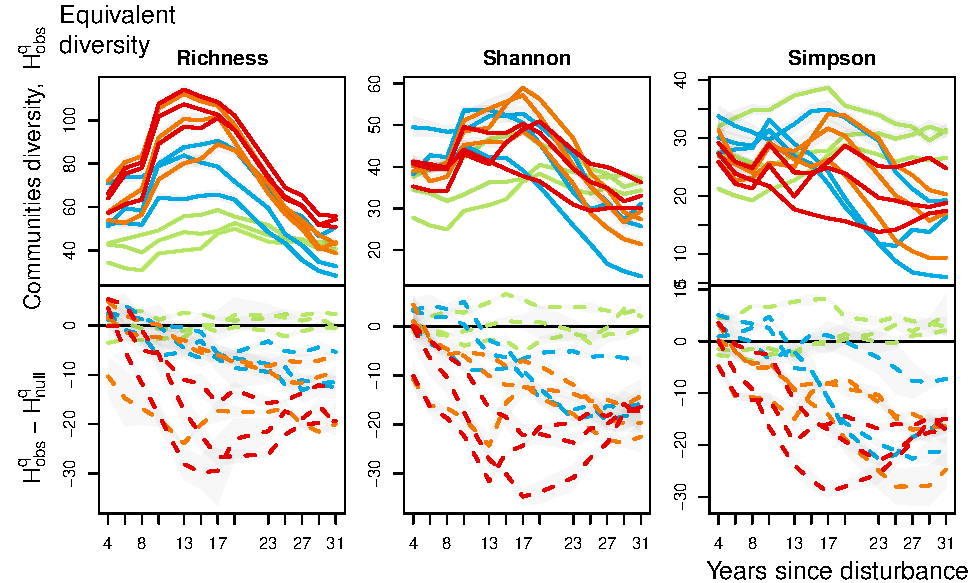
\includegraphics[width=0.8\linewidth]{RecruitmentTrajectories_files/figure-latex/Fig1-1} 

}

\caption{Trajectories for the 30 sampled years of Richness, Shannon and Simpson diversity for **(a)**  3-years laps punctual recruitment and **(b)** recruits accumulated since disturbance. Solid lines (green for control, blue for T1, orange for T2 and red for T3 disturbance treatments) correspond to the median observed after 50 iteration of the taxonomic uncertainty propagation, along with the 95\% confidence interval (grey envelope).}\label{fig:Fig1}
\end{figure}

\emph{Comparison to null model}

Punctual and accumulated recruitment diversity of order 0, 1 and 2 were
compared to a null recruitment model corresponding to the random
sampling of recruited trees holding constant the number of trees
recruited. For control plots the richness and evenness of observed
punctual recruitment were constantly equivalent or higher than obtained
with the null model \ref{fig:Fig2}. For the disturbed plots the richness
of observed punctual recruitment remained equivalent to this of the null
model but the evenness that was first equivalent or higher became and
remained lower than this of the null model from 10 years after
disturbance whenever the disturbance intensity.

\begin{figure}

{\centering 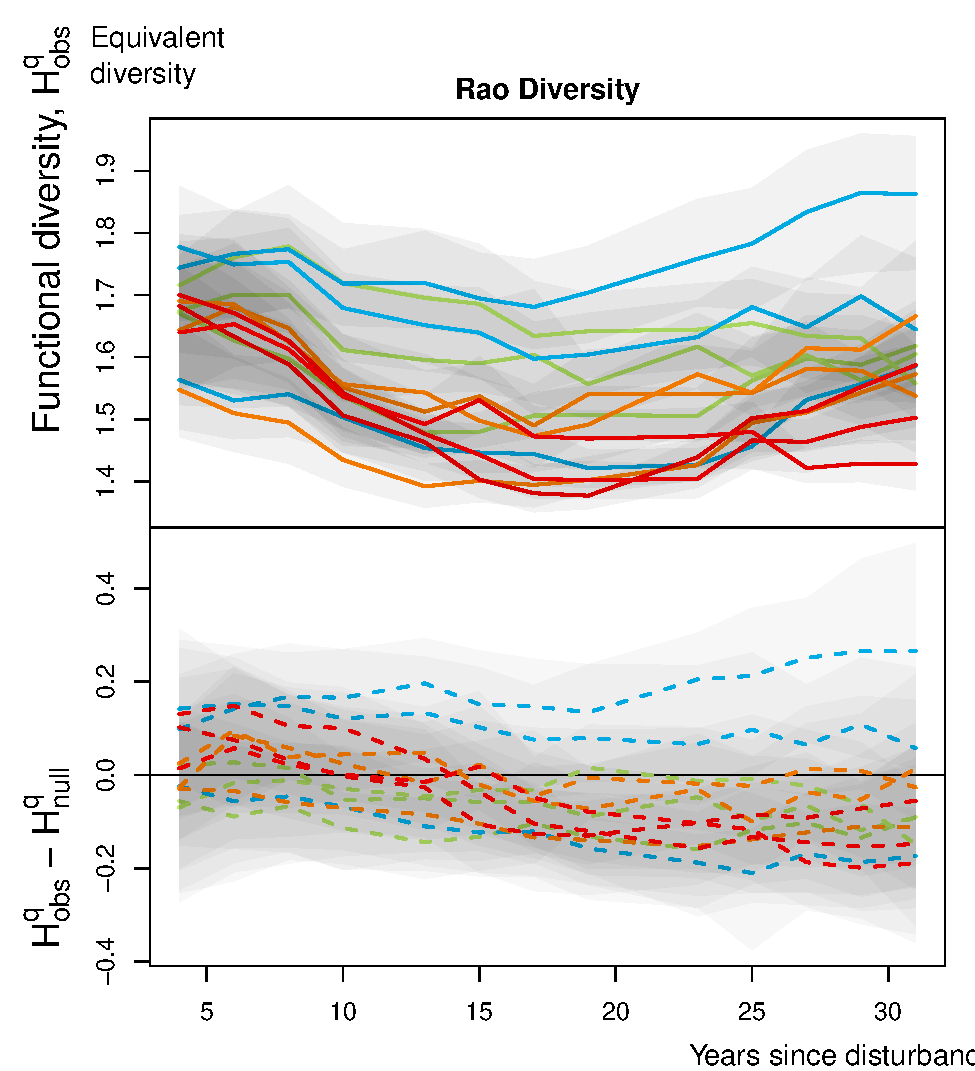
\includegraphics[width=0.8\linewidth]{RecruitmentTrajectories_files/figure-latex/Fig2-1} 

}

\caption{Punctual recruitment diversity trajectories for the Richness, Shannon and Simpson diversity compared to the null model trajectories. Values reported correspond to the median diversity observed after 50 repetition of the taxonomic uncertainty propagation. Solid lines correspond to the observed trajectories and dotted lines to the null model simulations.Line colors stand for the disturbance treatment with green for control, blue for T1, orange for T2 and red for T3 disturbance treatments.Values reported correspond to the median and 95\% confidence interval observed after 50 iterations of the taxonomic uncertainty propagation and null model simulation.}\label{fig:Fig2}
\end{figure}

In the same way as for punctual recruitment the richness and evenness of
accumulated recuits in control plots was equivalent or higher than
observed for the null model for all the post logging survey. On
disturbed plots the richness of accumulated recruits followed this of
the null model whereas the evenness, initially higher, became lower than
this of the null model after some time \ref{fig:Fig3}.

\begin{figure}

{\centering 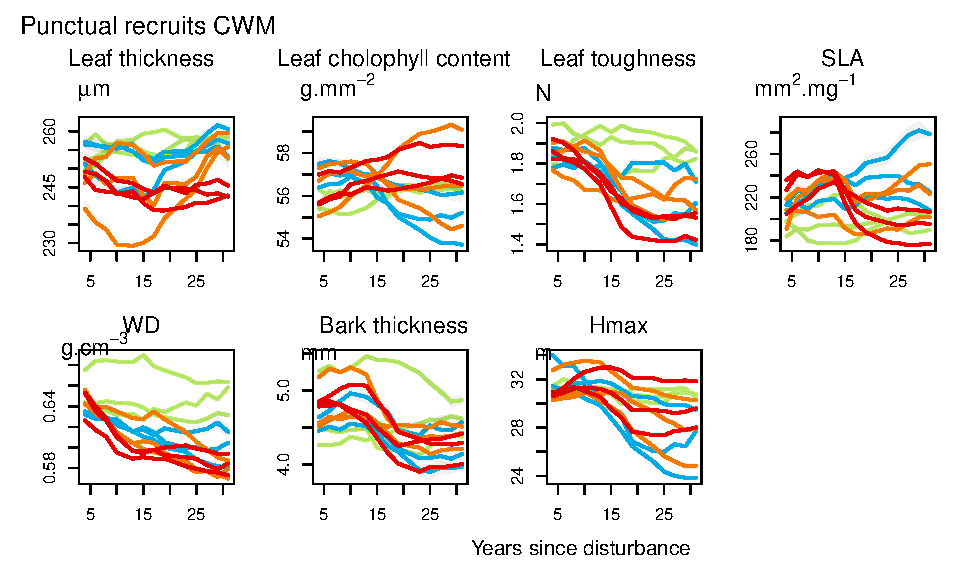
\includegraphics[width=0.8\linewidth]{RecruitmentTrajectories_files/figure-latex/Fig3-1} 

}

\caption{Accumulated recruitment diversity trajectories for the Richness, Shannon and Simpson diversity compared to the null model trajectories. Values reported correspond to the median diversity observed after 50 repetition of the taxonomic uncertainty propagation. Solid lines correspond to the observed trajectories and dotted lines to the null model simulations.Line colors stand for the disturbance treatment with green for control, blue for T1, orange for T2 and red for T3 disturbance treatments.Values reported correspond to the median and 95\% confidence intervalobserved after 50 iteration of the taxonomic uncertainty propagation and null model simulation..}\label{fig:Fig3}
\end{figure}

\emph{Recruitment functional diversity }

Punctual and accumulated recruitment diversity of order 0, 1 and 2 were
compared to a null recruitment model corresponding to the random shuffle
of complete set of traits value among species \ref{fig:Fig4}.

\begin{figure}

{\centering 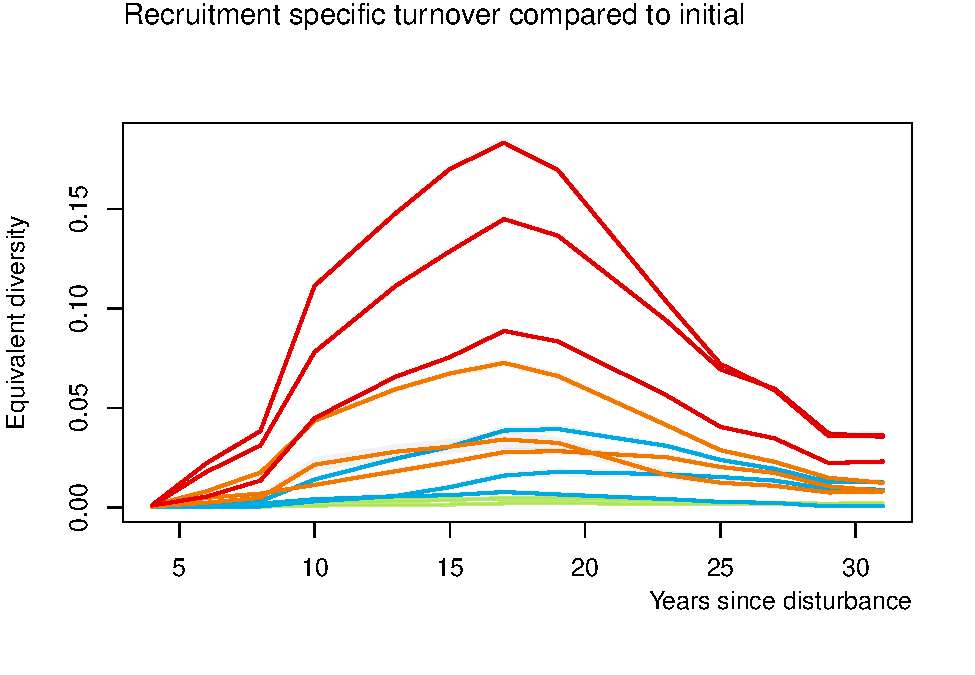
\includegraphics[width=0.5\linewidth]{RecruitmentTrajectories_files/figure-latex/Fig4-1} 

}

\caption{Functional diversity of punctual recruited trees from the considered functional traits. Values reported correspond to the plot-level median and the 95\% confidence interval obtained after 50 repetition of the taxonomic uncertainty propagation and the functional database gap-filling processes. Lines colors correspond to the logging treatment initially applied (green for control, blue for T1,orange for T2 and red for T3).}\label{fig:Fig4}
\end{figure}

Recruits functional diversity displayed a unimodal response to
disturbance with a maximum positively correlated to disturbance
intensity but with a time at maximum that was unrelated to the
disturbance treatment.

\emph{Recruitment traits weighted means}

The trajectories of recruited trees functional and life traits weighted
means showed the dominance after disturbance of species displaying large
exchange surface area and light tissues (high SLA, low leaf toughness
and low wood specific gravity) \ref{fig:Fig5}. all traits trajectories
dosplayed asymptotic CWM trajectories, except the SLA that displayed a
unimodal trajectory with a maximum positively correlated to disturbance
intensity and a time a maximum around ten years after disturbance
equivalent for all treatments.

\begin{figure}

{\centering 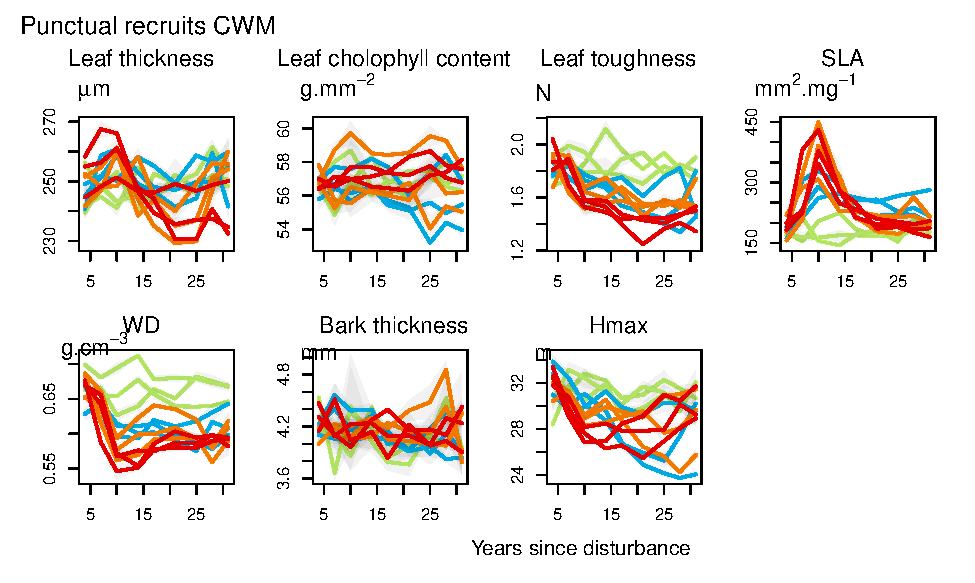
\includegraphics[width=0.8\linewidth]{RecruitmentTrajectories_files/figure-latex/Fig5-1} 

}

\caption{Community weighted means (CWM) of the four disturbance treatment for the four leaf traits, the two stem traits  and the specific Hmax. Values reported correspond to the plot-level median obtained after 50 repetition of the taxonomic uncertainty propagation and the functional database gap-filling processes. Lines colors correspond to the disturbance intensity (green for control, blue for T1,orange for T2 and red for T3).}\label{fig:Fig5}
\end{figure}

\textbf{Recruitment Turnover}

The abundance turnover of recruited trees compared to the initial stand
inventoried before exploitation remained even for the 30 sampled years
in the control plots \ref{fig:Fig6}. For the disturbed plot the
abundance turnover displayed a unimodal response to disturbance, with
maximum reached around 10 years after disturbance that was positively
correlated to the disturbance intensity. The turnover had returned close
to zero for all plots 30 years after disturbance.

\begin{figure}

{\centering 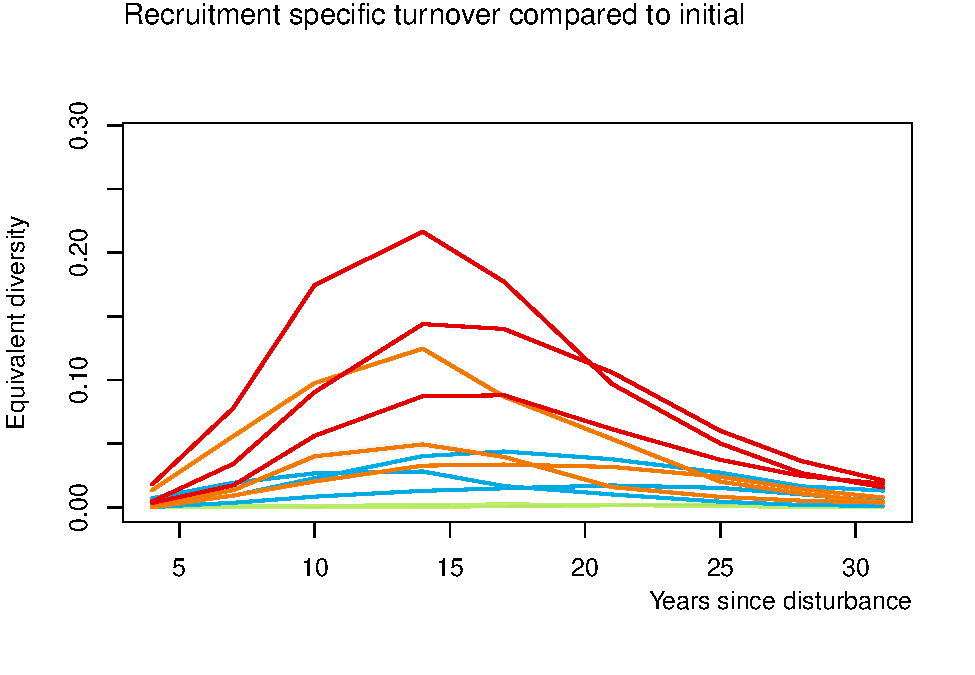
\includegraphics[width=0.5\linewidth]{RecruitmentTrajectories_files/figure-latex/Fig6-1} 

}

\caption{Trajectories over the 30 sampled years of the abundance-based turnover between recruited trees and intial stands before disturbance. 50 repetitions of the taxonomic propagation process returned the distribution of trunover values, grey envelopes correspond to the 0.025 and 0.975 percentiles and lines to the median in green for control, blue for T1,orange for T2 and red for T3).}\label{fig:Fig6}
\end{figure}

\section{Discussion}\label{discussion}

From the 30 years of forest dynamics survey in the Paracou station we
highlighted contrasting recruitment mechanisms between control and
post-disturbance tropical forests. The difference among treatments were
also significant which suggest an intensity threshold between the first
and second disturbance treatment and could involve gaps size, the
richness of exploited trees or the intervention density
\citep{Denslow1980}. \textgreater{} If we go for a model, maybe we can
test the most relevant parameter!?

Disturbance increases the recruitment rate which subsequently increased
the richness of recruitment but impaired its evenness, all the more so
that disturbance intensity was high. After disturbance the recruitment
was then dominated by a restricted pool of species and Shannon and
Simpson diversities decreased up to lower values than those of control
plots.

For the 15 first years following disturbance the recruitement seemed
driven by the growth of pre-disturbance saplings on hold of suitable
growth condition that benefitted from the environmental changes. This
translated by an increase in the functional diversity of recruits for
all disturbance intensity and an even distribution of functional traits.
According to the high increase of SLA CWM trajectory \ref{fig:Fig5}
right after disturbance these early recruited species would been
pionneers dominating the recruited community until 10 years after
disturbance.

After this first recruitment phase, in the case of low disturbance
intensity (T1 plots) the recruitment was highly nested within the
community in place and displayed a richness and evenness similar to
those of a random sampling null-model. This argues for the existence of
some recruitment limitation meaning the strive of a variety of species,
even when not the most fitted for the environmental context, because the
best competitors couldn't set in the disturbed area. The key role of
recruitment limitation in recovery dynamic was already highlighted for
low disturbance intensity in tropical wet forests
\citep{Hubbell1999, Sheil2003, Bongers2009} and supported the IDH as it
mitigates competitive exclusion and maintains some inferior competitiors
in the community. Recruitment and dispersal limitation are consistent
with the short dispersal distance observed for tropical trees, and it
was already highlighted in Paracou through the genetic clumping observed
for some pioneers \citep{Leclerc2015, Scotti2015a}.

In the case of high disturbance intensity, the species turnover was high
and the functional diversity decreased rapidly, along a recruitment
shift towards acquisitive functional strategies. This was particularly
marked for functional traits of the leaf and stem and for life history
traits (Leaf thickness, SLA, Wood Specific Gravity and Hmax) which
values represented a community of fast-growing species with a high
resources acquisition strategies
\citep{Wright2004, Chave2009b, Herault2011, Reich2014}. The time elpased
between disturbance and the significance of those functional and
diversity shifts suggests that the second recruitment phase stems from
the germination at the moment of the disturbance of seeds of the seed
bank. This recruitment would undergo a range of environmental filters
and thus restricting the pool of species recruited \citep{Molino2001}.

Eventually, we observed that disturbance induced particular recruitment
mechanisms but also set aside mechanisms at stake in natural plots.
Diversity of recruited community in undisturbed plots was higher than
this observed for a random-sampling null model, suggesting mechanisms
maintaining high diversity like negative density dependance
\citep{Harms2000}.

Previous studies already highlighted the significant diversity increase
of communities as a whole (Mirabel et al., in.prep.) that seemed
supported here by a shift in recruitment dynamics in favor of
acquisitive functional types \citep{TerSteege2001}.

After 30 years stands functional characteristics had recovered whenever
the disturbance intensity but significant taxonomic diversity difference
persisted when the disturbance intensity was high. Stands functioning
would then recover faster than taxonomic composition, which questions
the recovery and the role of functional redundancy regarding tropical
forests diversity. In any case, the recruitment turnover compared to
initial stand ended up close to zero. This argued for the maintenance or
for the recovery in relation to the stand \citep{Anderson2007} of the
before-disturbance environment. It also supported the convergence of
communities tree species taxonomic and functional composition in the
long term \citep{Li2016}. The communities recruited after disturbance
would then persist for more than 30 years as suggested by the remaining
difference among treatments but the initial recruitment dynamics seemed
restored at this point, ensuring communities resilience if no other
disturbance is applied. The different results of two studies on the same
site 10 years \citep{Molino2001} and 20 years \citep{Baraloto2012a}
already suggested the recovery towards initial taxonomic and functional
condition of the stands in revealing a decreasing proportion of pioneers
between the two periods. This is however only valid for a single
disturbance event, given that second recruitment phase assumed to rely
on the seed bank triggers a storage effect likely modifying the
trajectories after another disturbance event. We assume that in this
case the competitive exclusion among dormant life-stage (seeds or even
seedlings) would be harsher and bring more radical changes in the
recuitment composition and functional profile. Some functional shift
towards more acquisitive, small seeded and globally disturbance resitant
species building a more resilient community as it has been observed by
\citep{Haddad2008} who linked the persistence of species to their
ability to recover from disturbance which is the seed mass , growth rate
linked to WD and SLA for plants. Additionally to a somehow depleted seed
bank this strongly questioned the repeatability of observed trajectories
after other disturbance events.

Our long-term study of diversity trajectories after disturbance
desentangled the mechanisms underlying stands diversity. While, in
undisturbed forests, mechanisms like negative density dependence
enhanced species diversity, any disturbance induced new mechanisms
depending on the disturbance intensity. In any case, communities short
term response first reflected the growth of a variety of already grown
saplings which increased the taxonomic and functional evenness of the
community. When the disturbance was low, recruitment limitation was
balanced against environmental filters and induced a recruited community
mirroring the stand in place while selecting more acquisitive functional
types. When the disturbance was intense however the species turnover was
high and induced a recruited community significantly dominated by
acquisitive functional types and a restricted pool of species. In both
cases plots recruitment is specific, because it is determined by the
surrounding stand in case of low disturbance or because the competitive
exclusion randomly selected a restricted pool of species after intense
disturbance. At the landscape scale, then, disturbance increased the
diversity through the ``between patch'' difference
\citep{denslow1987, Chesson2000, Sheil2003}.

\begin{quote}
Connell 1978, refute the ``equal chance HP because trees don't recruit
equally'' Contrary to Hubbell and Molino: the question is ``do gaps
allow specific species to establish which would thrive otherwise?''
\citep{Sheil2003}. The turnover answers that yes it does
\end{quote}

\begin{center}\rule{0.5\linewidth}{\linethickness}\end{center}

%----------------------------------------------------------------------------------------
%	REFERENCE LIST
%----------------------------------------------------------------------------------------

\bibliographystyle{mee}
\makeatletter
\filename@parse{references.bib}
\bibliography{\filename@base}
\makeatother


%----------------------------------------------------------------------------------------

\end{document}
